%
% Document class
\documentclass[
8pt,
% handout,
]{beamer}
%
% Theme
\usetheme[
numbering=fraction,
% background=dark,
progressbar=head,
]{metropolis}
%
% Colors
\definecolor{murraygold}{RGB}{240,195,58}
\definecolor{murrayblue}{RGB}{2,8,69}
\setbeamercolor{normal text}{bg=white,fg=murrayblue}
\setbeamercolor{alerted text}{fg=murraygold}
\setbeamercolor{example text}{fg=murraygold}
%
% Detailed settings/packages
%
% General packages
\usepackage{textpos}
% \usepackage{fontspec}
%
% Location(s) of images
\graphicspath{{images/}}
%
% Fonts
\setsansfont[BoldFont={Fira Sans SemiBold}]{Fira Sans}
\setbeamerfont{title}{size=\huge}
\setbeamerfont{author}{size=\LARGE}
\setbeamerfont{date}{size=\normalsize}
\setbeamerfont{institute}{size=\normalsize}
\setbeamerfont{frametitle}{series=\mdseries}
%
% Margins
% \setbeamersize{text margin left=0.5cm,text margin right=0.5cm}
%
% Frame title logo
\makeatletter
\newlength{\frametitleheight}% <- NEW
\newsavebox{\beamer@titlebox}% <- NEW
\setbeamertemplate{frametitle}{%
  \ifbeamercolorempty[bg]{frametitle}{}{\nointerlineskip}%
  \@tempdima=\textwidth%
  \advance\@tempdima by\beamer@leftmargin%
  \advance\@tempdima by\beamer@rightmargin%
  \sbox{\beamer@titlebox}{% <- NEW
      \begin{beamercolorbox}[sep=0.3cm,left,wd=\the\@tempdima]{frametitle}
        \usebeamerfont{frametitle}%
        \vbox{}\vskip-1ex%
        \if@tempswa\else\csname beamer@fteleft\endcsname\fi%
        \strut\insertframetitle\strut\par%
        {%
          \ifx\insertframesubtitle\@empty%
          \else%
          {\usebeamerfont{framesubtitle}\usebeamercolor[fg]{framesubtitle}\insertframesubtitle\strut\par}%
          \fi
        }%
        \vskip-1ex%
        \if@tempswa\else\vskip-.3cm\fi% set inside beamercolorbox... evil here...
      \end{beamercolorbox}%
     }% <- NEW
     \usebox{\beamer@titlebox}% <- NEW
\settoheight{\frametitleheight}{\usebox{\beamer@titlebox}}% <- NEW
\addtolength{\frametitleheight}{\headheight}}
\makeatother
\addtobeamertemplate{frametitle}{}{%
  \begin{tikzpicture}[remember picture,overlay]
    \node[inner sep=0, outer sep=0, anchor= east,xshift=-2mm,yshift=-0.5*\frametitleheight] at (current page.north east) {\includegraphics[height=0.675cm, keepaspectratio]{murraystate-logo-shield.png}};
  \end{tikzpicture}}
%
% Progress bar width
\makeatletter
\setlength{\metropolis@progressinheadfoot@linewidth}{1pt}
\makeatother
%
% Footer
\setbeamertemplate{frame footer}{\vspace*{-5pt}\insertshorttitle\hfill\secname}
\setbeamerfont{page number in head/foot}{size=\tiny}
\setbeamercolor{footline}{fg=gray}
%
%%% Local Variables:
%%% mode: latex
%%% TeX-master: "git-tutorial"
%%% TeX-engine: xetex
%%% End:

%
% Document information
\title{Version Control}
\date{\today}
\author{Tyler D. Stoffel}
\institute{ENT 419: Senior Project I}
\titlegraphic{\vspace*{7.25cm}\includegraphics[width=4cm]{murraystate-logo-primary.png}}
%
% Start document
\begin{document}
\maketitle
%
\begin{frame}
  \frametitle{Last day of ENT 419}
  Some thoughts before we start:
  \begin{itemize}
    \item<2-> Remember to fill out the teacher/course evaluation (TCE) form. Fill in the survey on Canvas for 10 bonus report points.
    \item<3-> Ideas for improving the course are welcome.
          \begin{itemize}
            \item Better materials ordering system.
            \item A few in class activities relevant to design projects?
            \item Thoughts on the one-on-one meetings format?
          \end{itemize}
    \item<4-> Thank you!
  \end{itemize}
\end{frame}
%
\section{What is Version Control?}
%
\begin{frame}{Version control}
  \vspace*{\baselineskip}
  \begin{columns}
    %
    \begin{column}{0.6\linewidth}
      What is version control (VC)?
      \begin{itemize}
        \item The traditional way: New version? \\ \emph{File $\rightarrow$ Save as $\rightarrow$ myDocument\_v2.docx}
        \item The better way: Version control.
      \end{itemize}
      \onslide<2->{
        \begin{alertblock}{Version control}
          A system that records changes to files over time so that you can recall specific versions, merge changes, collaborate on developing the files, and more.
        \end{alertblock}
      }
      \vspace*{\baselineskip}
      \onslide<3->{
        Some programs that have version control built in:
        \begin{itemize}
          \item AutoCAD, OnShape, and SolidWorks
          \item Studio 5000
          \item Microsoft programs like Word, Excel, Teams (kind of)...
        \end{itemize}
      }
    \end{column}
    %
    \begin{column}{0.4\linewidth}
      \onslide<1->{
        \begin{figure}
          \centering
          
\includegraphics[width=3.5cm]{version-control-comic.png}
          \caption{The traditional way.}
        \end{figure}
      }
    \end{column}
    %
  \end{columns}
\end{frame}
%
\begin{frame}{What is \texttt{git}?}
  \vspace*{\baselineskip}
  \begin{columns}
    %
    \begin{column}{0.75\linewidth}
      \texttt{git} is the most popular version control software in the world.
      \begin{itemize}
        \item Created by Linux Torvalds, creator of Linux, in 2005.
        \item Free, open source distributed version control system.
        \item Mostly for code and text, but works for other types of files too.
        \item Developed for use on the command line, i.e. \\ \texttt{\small git commit "feat: Add third hot chocolate flavor to HMI"} \\ but many programs deal with that for you.
      \end{itemize}
      \onslide<2->{
        \vspace*{\baselineskip}
        Some of the power of \texttt{git}:
        \begin{itemize}
          \item \texttt{git log}: Visualize the changes made to all of your files.
          \item \texttt{git diff}: See details of what was changed.
          \item \texttt{git merge}: Automatically merge different versions of files together.
          \item \texttt{git checkout}: Revert your files to any previously committed state.
        \end{itemize}
      }
    \end{column}
    %
    \begin{column}{0.25\linewidth}
      \onslide<1->{
        \begin{figure}
          \centering
          
\includegraphics[width=2.25cm]{git-symbol.png}
        \end{figure}
        \vspace*{3\baselineskip}
        \begin{figure}
          \centering
          \hspace*{-\baselineskip}
          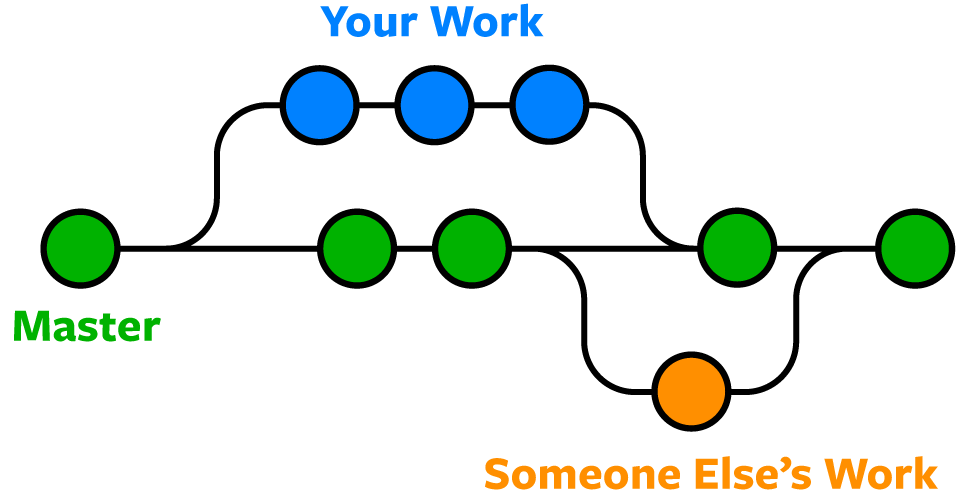
\includegraphics[width=3.5cm]{git-idea.png}
        \end{figure}
      }
    \end{column}
    %
  \end{columns}
\end{frame}
%
\begin{frame}{What is GitHub?}
  \vspace*{\baselineskip}
  \begin{columns}
    %
    \begin{column}{0.8\linewidth}
      GitHub is a cloud based \texttt{git} repository service.
      \begin{itemize}
        \item For profit, owned by Microsoft, with an annual revenue of \$1 billion.
        \item Used by 100 million developers.
        \item Usually used for public projects that everyone can use and develop themselves.
              \begin{itemize}
                \item Python, Go, Rust
                \item Linux, git itself
                \item Bitcoin
                \item Firefox, Brave Web Browser, Blender
                \item ChatGPT (soon)
              \end{itemize}
      \end{itemize}
    \end{column}
    %
    \begin{column}{0.2\linewidth}
      \onslide<1->{
        \begin{figure}
          \centering
          
\includegraphics[width=1.75cm]{github-symbol.png}
        \end{figure}
      }
    \end{column}
    %
  \end{columns}
  \pause
  \vspace*{\baselineskip}
  You've probably used GitHub before (save ZIP folder), but today we're talking about using it the powerful version control way.
\end{frame}
%
\begin{frame}
  \frametitle{Is \texttt{git} useful for EMT folks?}
  \pause
  Probably not.
  \pause
  \begin{itemize}
    \item Open source software is becoming more popular and widely used (e.g. the Click PLC).
    \item You're not software developers, but version control is a powerful tool for anything that uses scripts, code, or files.
    \item You can version control most anything that you do on a computer.
  \end{itemize}
\end{frame}
%
\begin{frame}
  \frametitle{\texttt{git} conventions}
  These are a few of the commands that are run in \texttt{git}, i.e. \texttt{git <command> ...}
  \begin{itemize}
    \item \texttt{clone}: Copy the files in the repository to your machine \emph{with} version control (not just download ZIP). \pause
    \item \texttt{commit}: A set of changes which you'd like to ``commit'' to the VC system. \pause
    \item \texttt{branch}: A set of separated commits given a name, usually meant for merging with the files on the main branch. \pause
    \item \texttt{(fork)}: Same as a branch, but distinguished because they're owned by you instead of the branch name. \pause
    \item \texttt{merge}: Tell \texttt{git} to merge a couple of branches together. \pause
    \item \texttt{diff}: Show the differences between a couple of branches or commits. \pause
    \item \texttt{log}: Show the history of changes on a branch. \pause
    \item \texttt{pull/push}: Accept or interject commits from/to the repository where the files are (GitHub). \pause
  \end{itemize}
\end{frame}
%
\section{Activity}
%
\begin{frame}
  \frametitle{Clone this repository}
  \begin{itemize}
    \item On the startup page of GitHub Desktop, click \emph{Clone a Repository from the internet}.
    \item Choose where you'd like to put the repository in the \emph{Local Path} box.
    \item Select \emph{URL}, and enter the URL for this repository: \url{https://github.com/tstoffel1/git-tutorial.git}.
    \item Click \emph{Clone}.
  \end{itemize}
  \begin{figure}
    \centering
    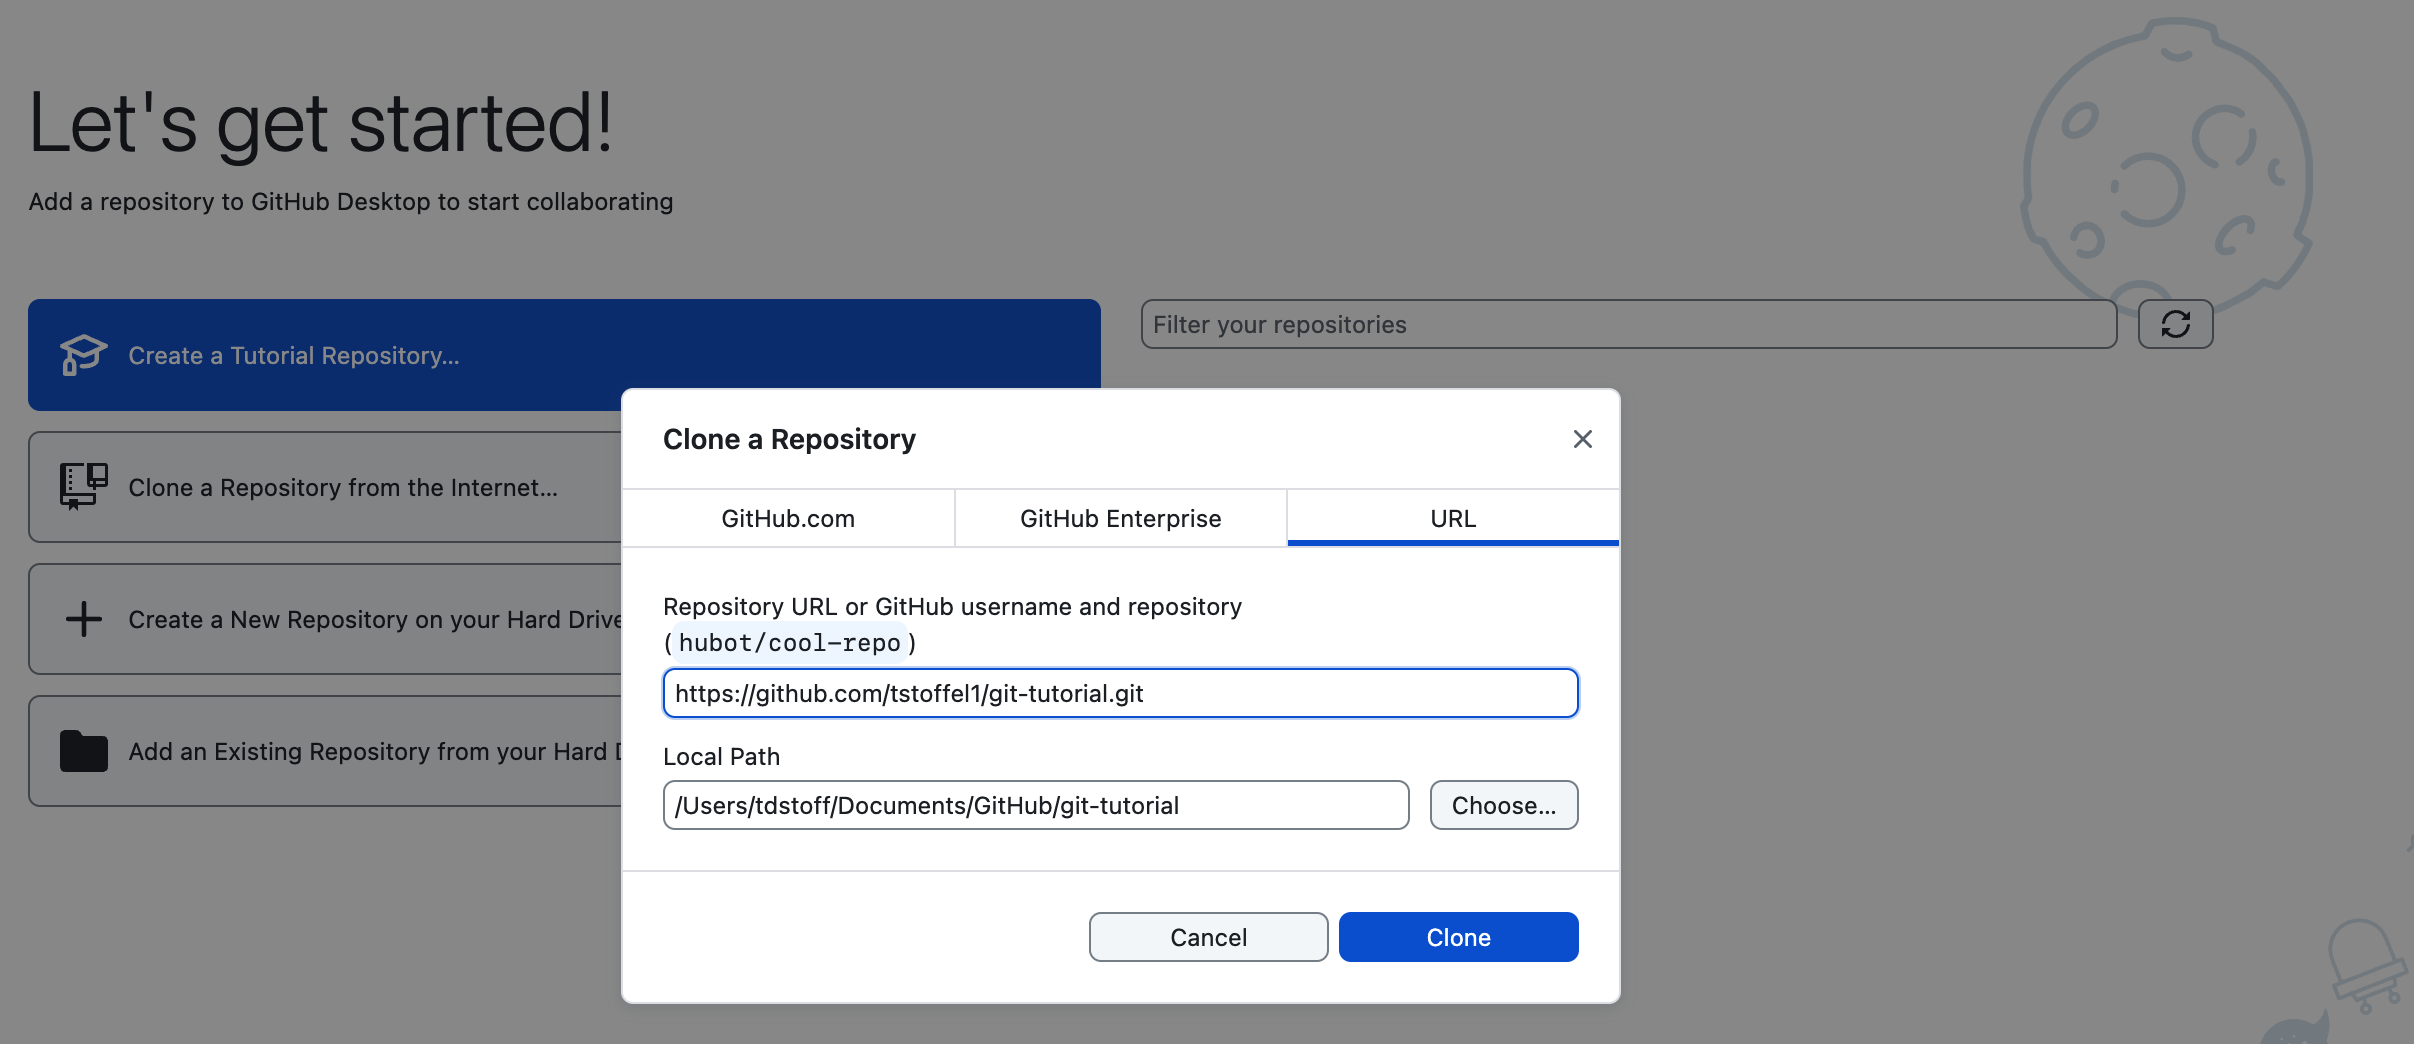
\includegraphics[width=0.9\linewidth]{activity-clone}
  \end{figure}
\end{frame}
%
\begin{frame}
  \frametitle{Part 1: Collaborate to spell check a document}
  \setlength{\leftmargini}{0cm}
  \begin{itemize}
    \item With your file explorer, open the file \texttt{proofread-this-file.txt} inside the folder that contains the repository.
    \item Find one spelling mistake and fix it with your text editor.
    \item Open GitHub Desktop again, navigate to the \emph{Changes} tab, and add a title which describes the change you made.
    \item Click \emph{create a fork} and then \emph{contribute to this repository}.
    \item Click \emph{commit to main}.
    \item Repeat this two more times (you don't have to fork the repository after the first time).
  \end{itemize}
  \begin{figure}
    \centering
    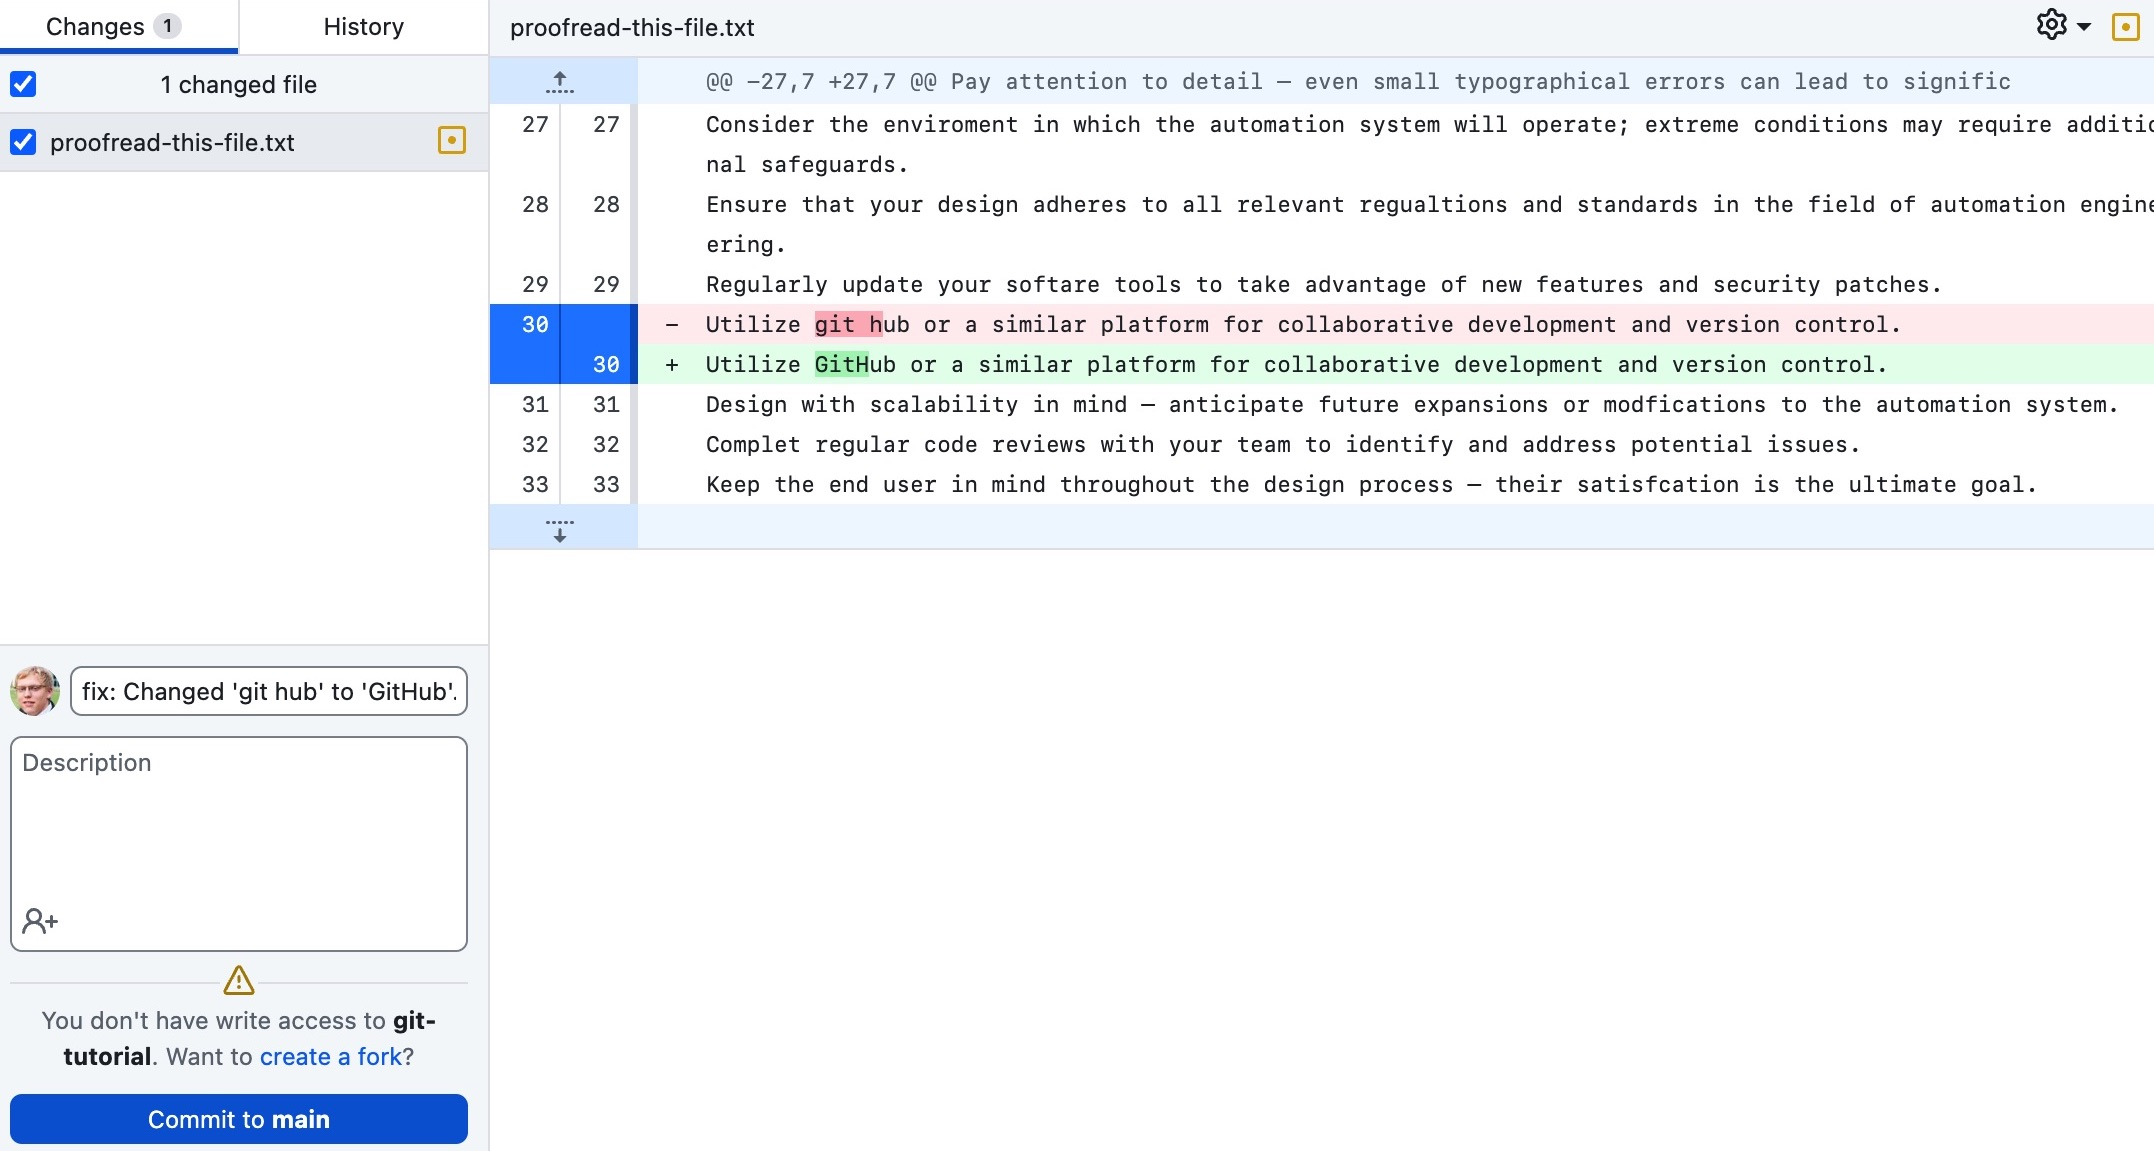
\includegraphics[width=0.8\linewidth]{activity-commit}
  \end{figure}
\end{frame}
%
\begin{frame}
  \frametitle{Part 2: Commit and label your Arduino code for the project}
  Commit your code into the repository:
  \begin{itemize}
    \item If you have your Arduino code from the project on your machine, use your file explorer to copy it into the \texttt{codes} folder inside the repository.
    \item If you don't have access the Arduino code, then create a text file with suffix \texttt{.ino} containing a comment line explaining you don't have it, e.g. \\ \texttt{// Our project group will not be uploading our Arduino code}.
    \item Open GitHub Desktop again, make sure your arduino code is checked in the \emph{changes} tab, add a title (e.g. ``committing our Arduino code'') and click \emph{commit to main}.
  \end{itemize}
  %
  \vspace*{\baselineskip}
  Add author information to your code:
  \begin{itemize}
    \item Open your Arduino code once more, and add an author line to the top of the code, e.g. \\ \texttt{// Authors: XXXX and YYYY}
    \item Commit this change as well with a title like ``Adding an author line to our code''.
  \end{itemize}
\end{frame}
%
\begin{frame}
  \frametitle{Push changes and submit a pull request}
  To push your commits to the fork you created under your username:
  \begin{itemize}
    \item Click \emph{Repository} $\rightarrow$ \emph{Push}.
  \end{itemize}
  To submit a request for the original repository owner (me) to merge those commits in:
  \begin{itemize}
    \item Click \emph{Branch} $\rightarrow$ \emph{Create pull request}.
    \item In the browser window that opens, fill in a title for your pull request with the names of your group members.
    \item Click \emph{Create pull request}.
  \end{itemize}
\end{frame}
%
\end{document}
%
%%% Local Variables:
%%% mode: latex
%%% TeX-engine: xetex
%%% TeX-master: t
%%% End:
